%-----------------------------------LICENSE------------------------------------%
%   This file is part of tikz_figures.                                         %
%                                                                              %
%   tikz_figures is free software: you can redistribute it and/or              %
%   modify it it under the terms of the GNU General Public License as          %
%   published by the Free Software Foundation, either version 3 of the         %
%   License, or (at your option) any later version.                            %
%                                                                              %
%   tikz_figures is distributed in the hope that it will be useful,            %
%   but WITHOUT ANY WARRANTY; without even the implied warranty of             %
%   MERCHANTABILITY or FITNESS FOR A PARTICULAR PURPOSE.  See the              %
%   GNU General Public License for more details.                               %
%                                                                              %
%   You should have received a copy of the GNU General Public License along    %
%   with tikz_figures.  If not, see <https://www.gnu.org/licenses/>.           %
%------------------------------------------------------------------------------%

% Use the standalone class for displaying the tikz image on a small PDF.
\documentclass[crop, tikz]{standalone}

% Import the tikz package to use for the drawing.
\usepackage{tikz}

% Begin the document.
\begin{document}

    % Begin the drawing.
    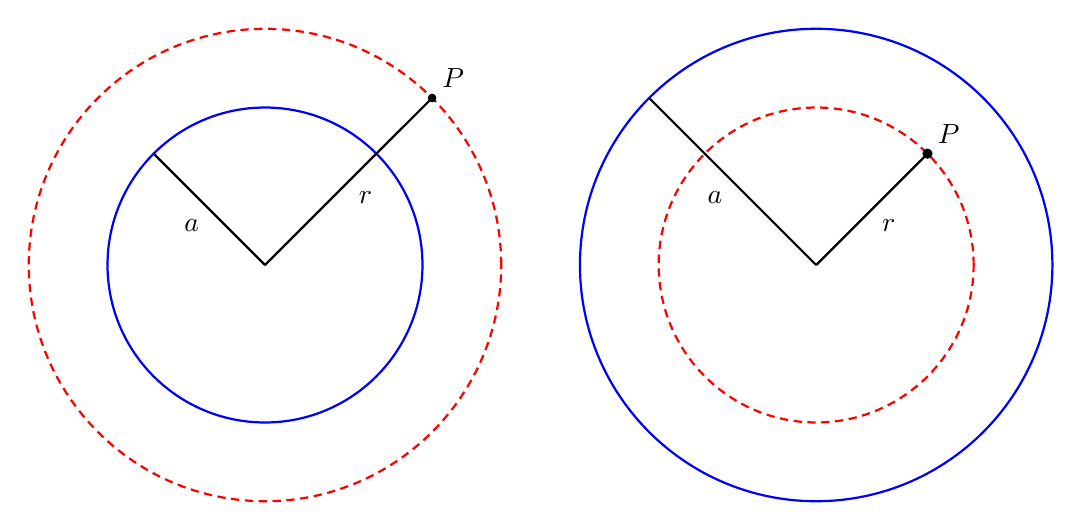
\begin{tikzpicture}[every path/.style = thick]

        % Solid blue circles.
        \begin{scope}[draw = blue]
            \draw (-3.5, 0.0) circle (2);
            \draw (3.5, 0.0) circle (3);
        \end{scope}

        % Dashed red circles.
        \begin{scope}[%
            draw = red,
            densely dashed
        ]
            \draw (-3.5, 0.0) circle (3);
            \draw (3.5, 0.0) circle (2);
        \end{scope}

        % Radial lines for the two blue and two red circles.
        \draw (-3.5, 0.0) to node[below left] {$a$} (-4.914, 1.414);
        \draw (-3.5, 0.0) to node[below right] {$r$} (-1.378, 2.121);
        \draw (3.5, 0.0) to node[below right] {$r$} (4.914, 1.414);
        \draw (3.5, 0.0) to node[below left] {$a$} (1.378, 2.121);

        % Mark the locations of P for the parts of the problem.
        \filldraw (-1.378, 2.121) circle (0.4mm) node[above right] {$P$};
        \filldraw (4.914, 1.414) circle (0.5mm) node[above right] {$P$};
    \end{tikzpicture}
\end{document}
